\section{Theorie}
\label{sec:Theorie}

In diesem Versuch werden die Suszeptibilitäten paramagnetischer Substanzen 
mit Hilfe einer Brückenschaltung bestimmt. Außerdem wird die Filterkurve 
des dabei verwendeten Selektivverstärkers untersucht. 

\subsection{Die magnetische Suszeptibilität}

Die magnetische Suszeptibilität $\chi$ ist eine dimensionslose Größe, die 
angibt, wie gut ein Material in einem externen Magnetfeld magnetisierbar ist,
d.h. wie sich die Magnetisierung $\vec{M}$ des Materials durch ein externes Magnetfeld 
ändert. Diese Größe ist im Allgemeinem von vielen Variablen abhängig (z.B. von der
magnetischen Feldstärke $\vec{H}$ und der Temperatur $T$) und tensoriell.

Allerdings nehmen die Suszeptibilitäten verschiedener Materiale unter Raumtemperatur und bei 
kleinen Magnetfeldern mit Feldstärken $\vec{B}$ kleiner einem Tesla näherungsweise
konstante Werte an, welches den linearen Ausdruck

\begin{equation}
    \vec{M} = \mu_0 \chi \vec{H}
\end{equation}

liefert. Mit dessen Hilfe lassen sich Materialien durch ihre magnetische Suszeptibilität 
unterscheiden. 

Stoffe mit einer Suszeptibilität $\chi < 0$ sind diamagnetisch, d.h. das Material 
magnetisiert in einem äußeren Magnetfeld entgegengesetzt zur Feldrichtung des Feldes,
sodass das innere Magnetfeld des Stoffvolumens schwächer ist.
Materialien mit einer Suszeptibilität $\chi > 0$ verhalten sich paramagnetisch, sodass
das Magnetfeld im Inneren des Stoffvolumens durch die Magnetisierung stärker ist, als 
das äußere anregende Magnetfeld.

Bei höheren Temperaturen verschwindet die Ordnung der Magnetisierung $\vec{M}$ nahezu
einheitlicher Richtung mit

\begin{equation}
    \chi \propto \frac{1}{T}
\end{equation}

antiproportional zur Umgebungstemperatur.

\subsection{Die Berechnung paramagnetischer Suszeptibilitäten}

Zur Berechnung der Suszeptibilität muss der Zusammenhang zwischen atomarem Drehimpuls
und magnetischem Momenten bekannt sein. Der Drehimpuls $\vec{J}$ eines Atoms setzt sich
aus dessen Bahnimpuls der Elektronenhülle $\vec{L}$, dem Gesamtspin $\vec{S}$
und dem für den Paramagnetismus vernachlässigbaren Kerndrehimpuls zusammen.
Dabei sind $\vec{L}$ und $\vec{S}$ Vektorsummen der einzelnen Elektronendrehimpulse
und -spins und ihnen können durch Erkenntnisse aus der Quantenmechanik folgende
magnetische Momente zugeordnet werden:

\begin{align}
    \vec{\mu}_L &= - \frac{\mu_\text{B}}{\hbar} \vec{L} \\
    \vec{\mu}_S &= - g_S \frac{\mu_\text{B}}{\hbar} \vec{S}
\end{align}

$\mu_\text{B}$ beschreibt dabei das Bohrsche Magneton und $g_S$ das
gyromagnetische Verhältnis.

\begin{figure} [H]!
    \centering
    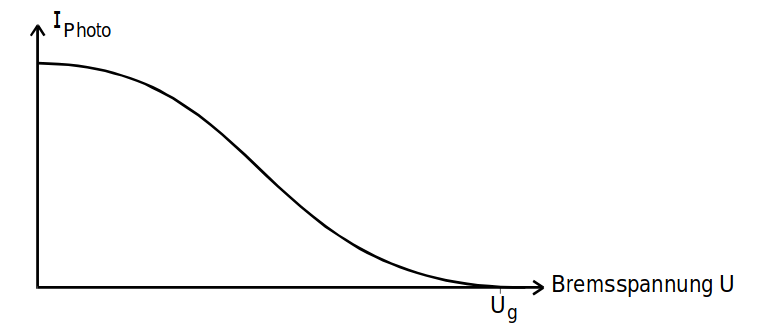
\includegraphics[scale=0.5]{content/bild3.png}
    \caption{Vektordiagramm der Drehimpulse im Elektron [1]}
    \label{fig:plot3}
  \end{figure}

Mit den Quantenzahlen der Drehimpulse $\vec{J}$ und $\vec{L}$ und des Spins $\vec{S}$
ergeben sich die Beträge

\begin{align}
    |\vec{\mu}_L| &= - \mu_\text{B} \sqrt{L\left(L+1\right)}\\
    |\vec{\mu}_S| &= - g_S \cdot \mu_\text{B} \sqrt{S\left(S+1\right)}
\end{align}

Zudem lässt sich aus Abbildung \ref{fig:plot3} die Beziehung

\begin{equation}
    |\vec{\mu}_J| = |\vec{\mu}_S| \cdot \text{cos}\left(\alpha \right) + 
    |\vec{\mu}_L| \cdot \text{cos}\left(\beta \right)
\end{equation}

ableiten und mit dem Kosinussatz zu 

\begin{equation}
    |\vec{\mu}_J| \approx \mu_\text{B} \cdot g_J \sqrt{J\left(J+1\right)}
\end{equation}

mit dem Lande-Faktor 

\begin{equation}
    g_J = \frac{3J(J+1) + [S(S+1) - L(L+1)]} {2 J(J+1)}
\end{equation}

vereinfachen.

Aus der Quantenmechanik geht des weiteren die Richtungsquantelung hervor, d.h.
der Winkel zwischen äußerem Magnetfeld und $\vec{\mu}_J$ ist nicht beliebig,
sondern es gilt die Beziehung 

\begin{equation}
    \mu_{J_Z} = - \mu_\text{B} \cdot g_J \cdot m
\end{equation}

für die Z-Komponente des magnetischen Moments $\mu_{J_Z}$ mit der ganzzahligen 
Orientierungsquantenzahl $m$, durch die es $2J+1$ Einstellungsmöglichkeiten
von $\vec{\mu}_J$ bezüglich des äußeren Magnetfeldes gibt. 

Über alle möglichen Einstellungen mit ihren jeweiligen Wahrscheinlichkeiten summiert,
ergibt sich für die Suszeptibilität der Zusammenhang

\begin{equation}
    \chi = \frac{\mu_0 \cdot \mu_\text{B}^2 \cdot g_J^2 \cdot N J (J+1)}{3kT}
    \label{eqn:theo}
\end{equation}

mit der Momentenanzahl pro Volumeneinheit $N$, der Boltzmannkonstante $k$ und der
Temperatur $T$.\\

In den Atomhüllen Seltener-Erd-Verbindungen sind sogenannte 4f-Elektronen dafür verantwortlich,
dass deren Paramagnetismus besonders gut beobachtbar ist. Für diese Elektronen und
den Gesamtdrehimpuls $\vec{J}$ gelten die Hundschen Regeln:

\begin{itemize}
    \item Die einzelnen Spins $\vec{s_i}$ summieren sich nach dem Pauli-Prinzip zum Gesamtspin
    $\vec{S} = \sum \vec{s_i}$ auf.
    \item Die einzelnen Bahndrehimpulse $\vec{l_i}$ summieren sich nach dem Pauli-Prinzip zum Maximaldrehimpuls 
    $\vec{L} = \sum \vec{l_i}$ auf.
    \item Der Gesamtdrehimpuls beträgt $\vec{J} = \vec{L} - \vec{S}$, wenn die Elektronenschale weniger und
    $\vec{J} = \vec{L} - \vec{S}$, wenn die Schale mehr als halbvoll besetzt ist.
\end{itemize}

\subsection{Messverfahren zur Bestimmung paramagnetischer Suszeptibilitäten}

Die Bestimmung der paramagnetischen Suszeptibilitäten basiert auf einer
Induktivitätsdifferenz $\Delta L$ zwischen einer mit einem Paramagneten 
befüllten oder unbefüllten Spule. Diese Spule ist hier Bestandteil der
Brückenschaltung aus Abbildung \ref{fig:plot1} und für hohe Spannungsfrequenzen
$\omega^2 L^2 >> R^2$ gilt die Beziehung 

\begin{equation}
    \Chi (\omega \to \infty) = \frac{4 F U_\text{Br}}{Q U_\text{Sp}} \; .
    \label{eqn:spannung}
\end{equation} 

Dabei beschreibt $F$ den Spulenquerschnitt, $Q$ den Probenquerschnitt und
$U_\text{Sp}$ die Speisespannung.

Für die Methode mit erneutem Abgleich der Brückenspannung 
kann außerdem die Beziehung 

\begin{equation}
    \Chi = \frac{2 \cdot \Delta R \cdot F}{R_3\cdot Q}
    \label{eqn:alternativ}
\end{equation}

verwendet werden, in der $\Delta R$ für die Differenz der Potentiometereinstellungen
steht.


















